\documentclass[border=5pt]{standalone}
\usepackage[T1]{fontenc}
\usepackage{lmodern}
\usepackage{pgfplots}
\usepgfplotslibrary{groupplots}
\pgfplotsset{compat=1.18}
\begin{document}
\sffamily
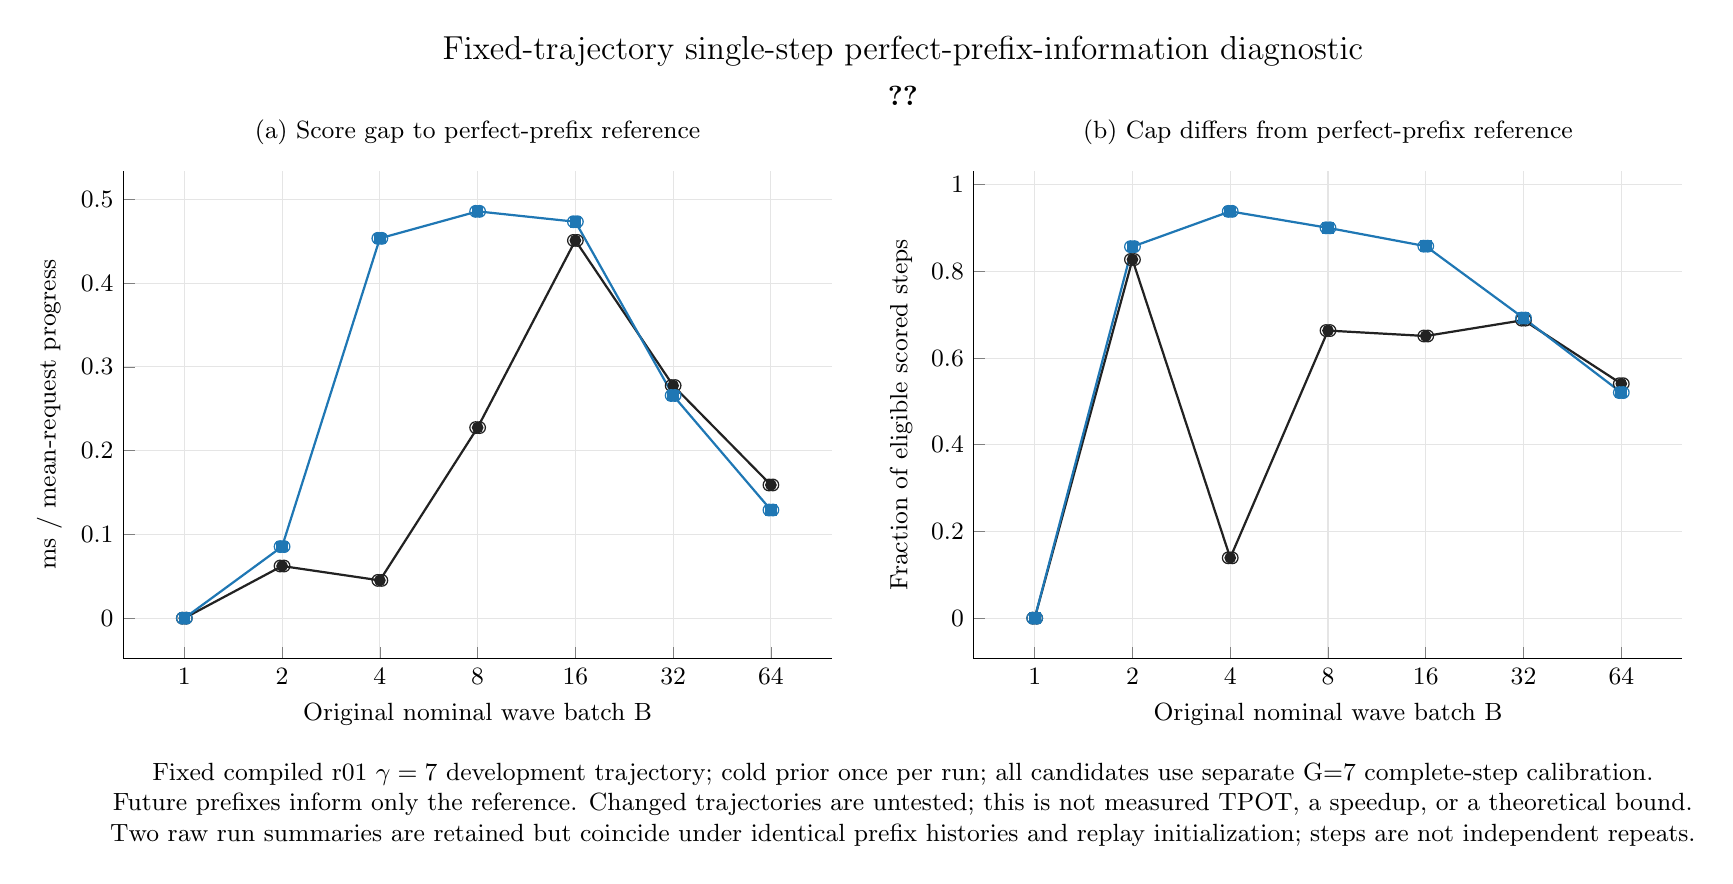
\begin{tikzpicture}
\definecolor{series0}{HTML}{222222}
\definecolor{series1}{HTML}{1f77b4}
\definecolor{series2}{HTML}{ff7f0e}
\definecolor{series3}{HTML}{2ca02c}
\definecolor{series4}{HTML}{d62728}
\definecolor{series5}{HTML}{9467bd}
\definecolor{series6}{HTML}{8c564b}
\definecolor{series7}{HTML}{e377c2}
\begin{groupplot}[group style={group size=2 by 1,horizontal sep=1.8cm},width=9.0cm,height=6.2cm,scale only axis,grid=major,grid style={gray!20},axis lines*=left,tick label style={font=\small},label style={font=\small},title style={font=\small},unbounded coords=jump]
\nextgroupplot[title={(a) Score gap to perfect-prefix reference},xlabel={Original nominal wave batch B},ylabel={ms / mean-request progress},xtick={1,2,4,8,16,32,64},xticklabels={1,2,4,8,16,32,64},xmode=log,log basis x=2,minor x tick num=0,scaled y ticks=false,yticklabel style={/pgf/number format/fixed,/pgf/number format/precision=2},legend columns=2,legend to name=sharedlegend,legend style={draw=none,font=\small,/tikz/every even column/.append style={column sep=8pt}}]
\addplot+[color=series0,mark=*,mark size=1.7pt,mark options={fill=series0,draw=series0},line width=0.8pt] coordinates {(1,0) (2,0.0622706887403) (4,0.045120113414) (8,0.22752761579) (16,0.450931069896) (32,0.27764594563) (64,0.159021570155)};
\addlegendentry{Replayed pre-step cap}
\addplot+[only marks,forget plot,color=series0,mark=o,mark size=2.1pt,mark options={fill=white,line width=0.45pt}] coordinates {(0.986097544263,0) (1.01409845894,0) (1.97219508853,0.0622706887403) (2.02819691788,0.0622706887403) (3.94439017705,0.045120113414) (4.05639383575,0.045120113414) (7.8887803541,0.22752761579) (8.11278767151,0.22752761579) (15.7775607082,0.450931069896) (16.225575343,0.450931069896) (31.5551214164,0.27764594563) (32.451150686,0.27764594563) (63.1102428328,0.159021570155) (64.9023013721,0.159021570155)};
\addplot+[color=series1,mark=square*,mark size=1.7pt,mark options={fill=series1,draw=series1},line width=0.8pt] coordinates {(1,0) (2,0.0854449149448) (4,0.453427478338) (8,0.485649738005) (16,0.473270993483) (32,0.265835424512) (64,0.129113406079)};
\addlegendentry{Recorded cap7}
\addplot+[only marks,forget plot,color=series1,mark=o,mark size=2.1pt,mark options={fill=white,line width=0.45pt}] coordinates {(0.986097544263,0) (1.01409845894,0) (1.97219508853,0.0854449149448) (2.02819691788,0.0854449149448) (3.94439017705,0.453427478338) (4.05639383575,0.453427478338) (7.8887803541,0.485649738005) (8.11278767151,0.485649738005) (15.7775607082,0.473270993483) (16.225575343,0.473270993483) (31.5551214164,0.265835424512) (32.451150686,0.265835424512) (63.1102428328,0.129113406079) (64.9023013721,0.129113406079)};
\nextgroupplot[title={(b) Cap differs from perfect-prefix reference},xlabel={Original nominal wave batch B},ylabel={Fraction of eligible scored steps},xtick={1,2,4,8,16,32,64},xticklabels={1,2,4,8,16,32,64},xmode=log,log basis x=2,minor x tick num=0,scaled y ticks=false,yticklabel style={/pgf/number format/fixed,/pgf/number format/precision=2}]
\addplot+[color=series0,mark=*,mark size=1.7pt,mark options={fill=series0,draw=series0},line width=0.8pt] coordinates {(1,0) (2,0.827285129604) (4,0.139186295503) (8,0.66341991342) (16,0.650900900901) (32,0.6875) (64,0.540816326531)};
\addplot+[only marks,forget plot,color=series0,mark=o,mark size=2.1pt,mark options={fill=white,line width=0.45pt}] coordinates {(0.986097544263,0) (1.01409845894,0) (1.97219508853,0.827285129604) (2.02819691788,0.827285129604) (3.94439017705,0.139186295503) (4.05639383575,0.139186295503) (7.8887803541,0.66341991342) (8.11278767151,0.66341991342) (15.7775607082,0.650900900901) (16.225575343,0.650900900901) (31.5551214164,0.6875) (32.451150686,0.6875) (63.1102428328,0.540816326531) (64.9023013721,0.540816326531)};
\addplot+[color=series1,mark=square*,mark size=1.7pt,mark options={fill=series1,draw=series1},line width=0.8pt] coordinates {(1,0) (2,0.857025920873) (4,0.938436830835) (8,0.900432900433) (16,0.858108108108) (32,0.692307692308) (64,0.520408163265)};
\addplot+[only marks,forget plot,color=series1,mark=o,mark size=2.1pt,mark options={fill=white,line width=0.45pt}] coordinates {(0.986097544263,0) (1.01409845894,0) (1.97219508853,0.857025920873) (2.02819691788,0.857025920873) (3.94439017705,0.938436830835) (4.05639383575,0.938436830835) (7.8887803541,0.900432900433) (8.11278767151,0.900432900433) (15.7775607082,0.858108108108) (16.225575343,0.858108108108) (31.5551214164,0.692307692308) (32.451150686,0.692307692308) (63.1102428328,0.520408163265) (64.9023013721,0.520408163265)};
\end{groupplot}
\path (group c1r1.north west) -- node[above=1.2cm,font=\large] {Fixed-trajectory single-step perfect-prefix-information diagnostic} (group c2r1.north east);
\path (group c1r1.north west) -- node[above=0.7cm] {\ref{sharedlegend}} (group c2r1.north east);
\path (group c1r1.south west) -- node[below=1.2cm,align=center,font=\small] {Fixed compiled r01 $\gamma=7$ development trajectory; cold prior once per run; all candidates use separate G=7 complete-step calibration.\\Future prefixes inform only the reference. Changed trajectories are untested; this is not measured TPOT, a speedup, or a theoretical bound.\\Two raw run summaries are retained but coincide under identical prefix histories and replay initialization; steps are not independent repeats.} (group c2r1.south east);
\end{tikzpicture}
\end{document}
